%%%%%%%%%%%%%%%%%%%%%%%%%%%%%%%%%%%%%%%%%%%%%%%%%%%%%%%%%%%%%%%%%%%%%%%%%%%%%%%%
%2345678901234567890123456789012345678901234567890123456789012345678901234567890
%        1         2         3         4         5         6         7         8

\documentclass[letterpaper, 10 pt, conference]{ieeeconf} 
%\usepackage{times}
\usepackage{algorithmic}
\usepackage{algorithm}
\usepackage{subcaption}
%\documentclass[a4paper, 10pt, conference]{ieeeconf}      % Use this line for a4 paper

% See the \addtolength command later in the file to balance the column lengths
% on the last page of the document

% The following packages can be found on http:\\www.ctan.org
%\usepackage{graphics} % for pdf, bitmapped graphics files
%\usepackage{epsfig} % for postscript graphics files
%\usepackage{mathptmx} % assumes new font selection scheme installed
%\usepackage{times} % assumes new font selection scheme installed
%\usepackage{amsmath} % asRRTLearnICRAsumes amsmath package installed
%\usepackage{amssymb}  % assumes amsmath package installed
\usepackage{mathtools}
\usepackage{amsmath}
%\usepackage{amsfonts}
\usepackage{color}
\usepackage{amssymb}
\DeclareMathOperator*{\argmin}{\arg\!\min} 
\DeclareMathOperator*{\argmax}{\arg\!\max} 
\usepackage[normalem]{ulem}
\useunder{\uline}{\ul}{}

% \title{\LARGE \bf
% Rapidly Exploring Learning Trees
% }
\IEEEoverridecommandlockouts                              % This command is only needed if 
                                                          % you want to use the \thanks command

\overrideIEEEmargins  

\title{\LARGE \bf
Acquiring Social Interaction Behaviours for Telepresence Robots\\via Deep Learning from Demonstration 
}


\author{Kyriacos Shiarlis$^{1}$, Joao Messias$^{1}$, and Shimon Whiteson$^{2}$% <-this % stops a space
% \thanks{*This work was not supported by any organization}% <-this % stops a space
\thanks{$^{1}$Informatics Institute, University of Amsterdam, The Netherlands,
         {\tt\small \{k.c.shiarlis,j.messias\}@uva.nl}}%
\thanks{$^{2}$Department of Computer Science, University of Oxford, United Kingdom,
         {\tt\small shimon.whiteson@cs.ox.ac.uk}}%
}



% \author{Kyriacos Shiarlis \\
% University of Amsterdam \\
% k.c.shiarlis@uva.nl
% \And 
% Joao Messias \\
% University of Amsterdam \\ 
% jmessias@uva.nl 
% \And
% Shimon Whiteson \\
% University of Oxford \\
% shimon.whiteson@cs.ox.ac.uk 
% }
\newcommand{\jm}[1]{\textcolor{blue}{Joao: #1}}

\newcommand{\sw}[1]{\textcolor{red}{SW: #1}}
\newcommand{\ks}[1]{\textcolor{green}{KS: #1}}


\begin{document}

\maketitle

\thispagestyle{empty}
\pagestyle{empty}


%%%%%%%%%%%%%%%%%%%%%%%%%%%%%%%%%%%%%%%%%%%%%%%%%%%%%%%%%%%%%%%%%%%%%%%%%%%%%%%%
\begin{abstract}
As robots begin to inhabit public and social spaces, it is increasingly important to ensure that they behave in a socially appropriate way. However, manually coding social behaviours is prohibitively difficult since social norms are hard to quantify.  Therefore, \emph{learning from demonstration} (LfD) \cite{argall2009survey}, wherein control policies are inferred from demonstrations of correct behaviour, is a powerful tool for helping robots acquire social intelligence. In this paper, we propose a deep learning approach to learning social behaviours from demonstration.  We apply this method to two challenging social tasks for a semi-autonomous telepresence robot.  Our results show that our approach outperforms both a naive controller and \emph{gradient boosting regression}.  Furthermore, ablation experiments confirm that each element of our method is essential to its success.
\end{abstract}

%%%%%%%%%%%%%%%%%%%%%%%%%%%%%%%%%%%%%%%%%%%%%%%%%%%%%%%%%%%%%%%%%%%%%%%%%%%%%%%%
\section{Introduction}


In recent years, robots have been migrating out of conventional, constrained, industrial environments and into more social and less structured ones such as museums \cite{thrun1999minerva}, airports \cite{triebel2015spencer}, restaurants \cite{qing2010research} and care centres \cite{shiarlis2015teresa}. This shift poses countless challenges for robotics, from hardware  to high-level behaviour design.  A particularly vexing challenge is to imbue robots with sufficient \emph{social intelligence}, i.e., to ensure that they respect social norms when interacting with humans or completing tasks in the presence of humans.  For example, a robot facing a group of people must maintain an appropriate distance, orientation, level of eye contact, etc.

Because socially acceptable behaviour is difficult to describe procedurally, it is typically infeasible to manually code social intelligence.  Furthermore, even traditional approaches to learning behaviour, such as \emph{reinforcement learning}, are not practical because social norms are too difficult to quantify in the form of a reward or cost function.

%One challenge that arises in social environments is that of personalisation. For example the social distance and pose that a robot should maintain when facing a group of people might vary from place to place \cite{joosse2014cultural}. This means that the robot's designer's should design the robot such that parameters can be changed. Additionally, social behaviors might be hard to program manually, for example how a robot should approach a group of people is still the subject of ongoing research \cite{vroon2015dynamics}. Finally, it would be favourable if non-roboticists could program different robot behaviours as they please without a technical expert. 

A compelling alternative is \emph{learning from demonstration} (LfD), wherein control policies are inferred from example demonstrations of correct behaviour.  Because demonstrating socially appropriate behaviour is typically straightforward for humans, obtaining the data needed to learn social intelligence from demonstration is highly feasible. In addition, many different behaviours can be learned with the same LfD algorithm, allowing non-roboticists to program personalised robotic behaviours simply by demonstrating the task.%, an idea already exploited in industry with robots such as Baxter \footnote{www.rethinkrobotics.com} 

% is a powerful tool. Instead of programming behaviours manually LfD, employes human demonstrations along with learning algorithms, whose aim is to extract the program from the data. This means that complex social behaviours that would require carefuly crafted programs can be learned from demonstrations. More importantly, if the learning algorithms are sufficiently generic, they can be used to learn a variety of tasks for a specific application. This in turn means that demonstrations no longer need to be coming from a roboticist, but from anyone that is capable on controlling the robot. 

However, to be practical for real robots, LfD must overcome some challenges of its own.  First, it must learn control policies that are robust to inevitable errors in the robot's perception system.  For example, a social robot must be able to detect and localise people in its environment.  If errors in such perception occur while demonstration data is being collected, then the LfD algorithm may misinterpret the demonstration, e.g., by inferring that the robot was avoiding a person when actually no person was present.  Furthermore, if perception errors occur when the learned policy is deployed, then the robot may behave incorrectly.

A second challenge is to cope with the dynamic size of the perceptual input.  A robot that interacts with a group of people must be able to cope with groups of different sizes, and even people coming and going within a single conversation.  This is a poor match for most LfD methods, which assume observations in the form of fixed-length feature vectors.

Third, in order to be useful for non-experts, the LfD algorithm must be sufficiently generic. In other words, it should be able to learn a wide set of behaviours with a single algorithm, by varying only the data. 

%To achieve this however, LfD would needs to surpass a few challenges of its own. Firstly as mentioned above, the learning algorithms need to be sufficiently generic. If for example we are learning low level behaviors for a mobile robot, we should be able to learn a wide set of behavious with a single learning algorithm, only by varying the data. Failure to do so would mean that each behaviour would require us to program a different learning procedure which would take away much of the benefit of LfD. 

%Another challenge that is especially relevant in social robotics is the robustness of the robot's perception, due to the highly unstructured nature of the environment and limitations in the sensors. Noisy perception can greatly confuse LfD methods if those are not designed to be robust to it. As an example consider a social robot that is supposed to follow a person in a relatively crowded space. The robot must maintain the belief about the identity of the person it is following, furthermore it should be robust to false positive people detections within the environment. Failure to do so would result in the robot 'misunderstaning' what the demonstrations wanted to show.

In this paper, we propose \emph{deep behavioural social cloning} (DBSoC), a new LfD architecture that overcomes these challenges.  \emph{Behavioural cloning} is an approach to LfD in which a control policy is directly inferred using supervised learning, i.e., the demonstrated actions are treated as labels for the corresponding observations, and a mapping from observations to actions is learned.  By leveraging the power of deep learning, DBSoC makes behavioural cloning practical for social robotics.  In particular, DBSoC `paints' the output of the robot's person detection and localisation system onto a 2D `image', which is then fed to a convolutional neural network.  In this way, DBSoC can cope elegantly with varying numbers of people, as well as automatically discover useful features for selecting actions.  In addition, DBSoC employs \emph{long short-term memory} (LSTM) network layers, allowing it to condition action selection on its history of observations and thus filter out transient perceptual errors.

%Recent advancements in Deep Learning allow computers and robots to perform many learning tasks with a single neural network architecture [atari],[sensimotor]. In addition certain methods within the field have shown robustness to noisy time-dependent inputs allowing the machine to learn many aspects of the environment that previous methods would assume a hand coded model for. For example the system might learn to ignore sensor readings or detections with certain characteristics if that is found to degrade the performance of the system.

We apply DBSoC to learn two social behaviours for a semi-autonomous holonomic telepresence robot. In the first task, the robot must continually adjust its position and orientation while interacting with a group of people of dynamic size and position.  In the second task, the robot must follow two people as their relative positions change.

We evaluated DBSoC on these two tasks by deploying the learned policies on a real telepresence robot and having it interact with actual human subjects.  Our quantitative and qualitative results show that DBC outperforms both a naive controller and a \emph{gradient boosting regression} baseline.  Furthermore, ablation experiments confirm that each element of DBC is essential to its success.

% has to do with reconfiguration of the robot when interacting with a group. Taking that is, the correct body pose in the presence of a group of people of changing size and position. The second behaviour is following two people in abitrary formation. The rest of the paper is organised as follows. Section 2 describes the behaviours we wish to learn, summarises related work in the field and describes the experiments performed to collect the required data. Section 3 explains the challenges inherent in the tasks and the collected data. Through these challenges we explain the design choices for our neural network architecture. Section 4 describes quantitative and qualitative evaluation of our system against baselines. Section 5 concludes the paper and details our plans for further work.

\section{Problem Statement \label{sec:related_work}}

In this paper, we consider two social tasks for a telepresence robot.  Such a robot acts as an avatar for a remotely present \emph{pilot} controlling the machine.  While telepresence robots are typically manually controlled, we aim to automate low-level control so that the pilot need only give high-level commands telling the robot, e.g., to follow a particular person or support a conversation with appropriate body poses.  Because telepresence robots are inherently social, and especially since they represent their pilots as avatars, it is essential that any learned behaviour be socially appropriate. In this section, we describe the two particular telepresence tasks considered in this paper, and the demonstration data we collected.  For both tasks, we assume the robot is equipped with an imperfect person detection and localisation system.  We also assume it is operating in an unstructured in environment containing a dynamic number of people, some of whom may not be involved in the pilot's conversation.

\subsection{Group Reconfiguration Task} 

In the first task, the robot must maintain a socially appropriate position and orientation as the location, position, and size of the group with which the pilot is interacting changes.  To do so, the robot must distinguish people who part of the conversation from those who are merely in the scene. Though this task, shown diagrammatically in Figure \ref{fig:static}, looks deceptively simple, manually coding such behaviour, or even deciding on what features such behaviour should condition, is quite difficult in practice, making it an ideal application for LfD.

Previous work has considered what effect robot repositioning following a change in a conversation group's size and shape has on the people in that group \cite{kuzuoka2010reconfiguring,vroon2015dynamics}. Here, we consider how to automate such repositioning using LfD.  Other work considers how to detect groups of people in crowded environments \cite{lau2010multi} and then interact with them.  In our approach, groups are not explicitly detected, though the learned control policy may implicitly do so when deciding how to act.

	\begin{figure}[tbh]
%	\hspace{-5cm}
	\centering
      \begin{subfigure}[b]{0.39\columnwidth}
    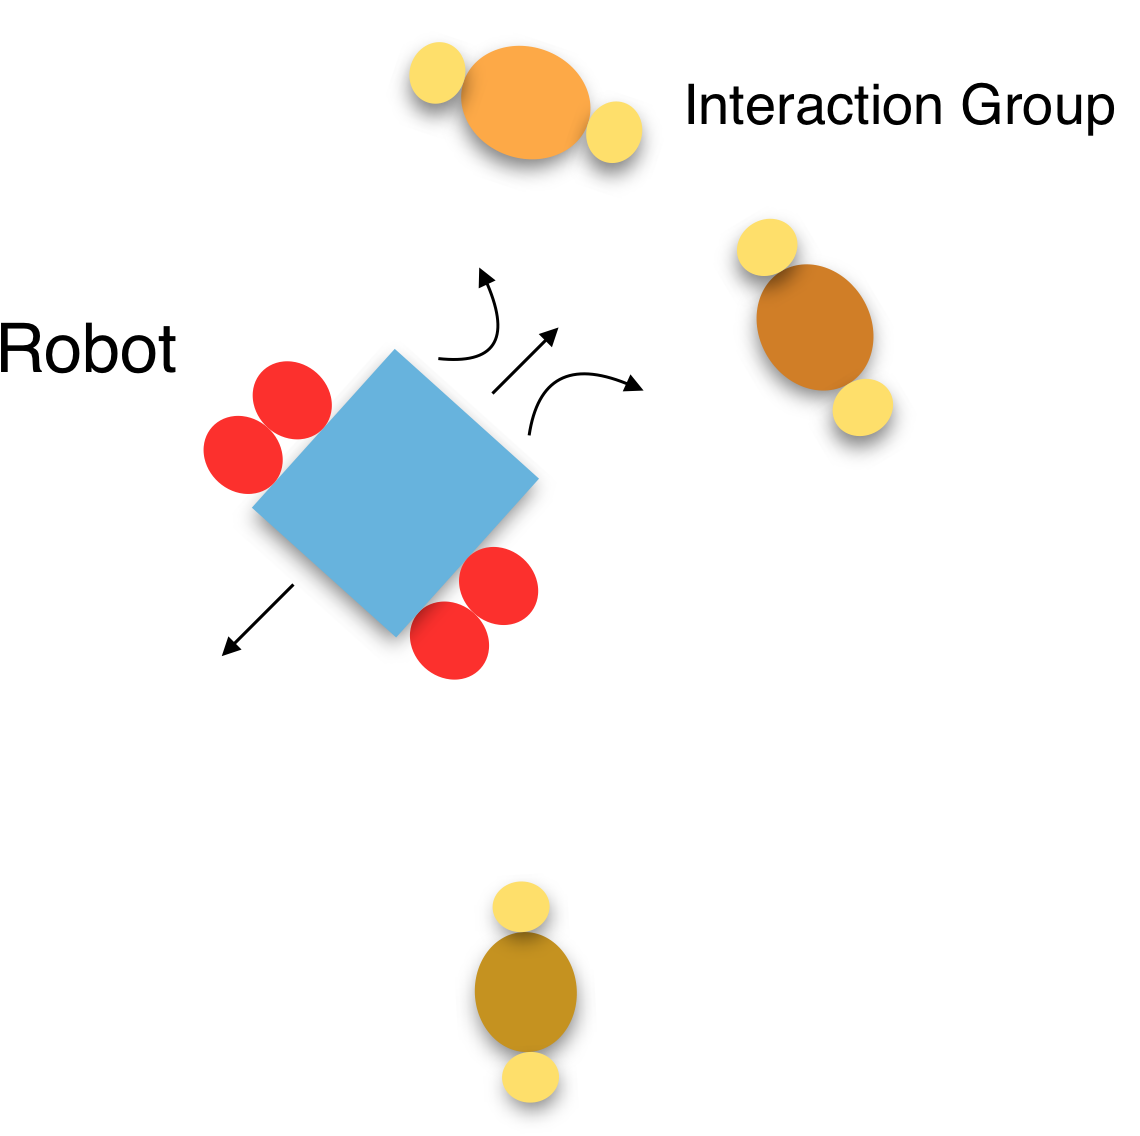
\includegraphics[scale = 0.15]{images/static.png}
    \caption{Group Reconfiguration}
    \label{fig:static}
  \end{subfigure}
  \hspace{10mm}
  \begin{subfigure}[b]{0.39\columnwidth}
  \hspace{4mm}
    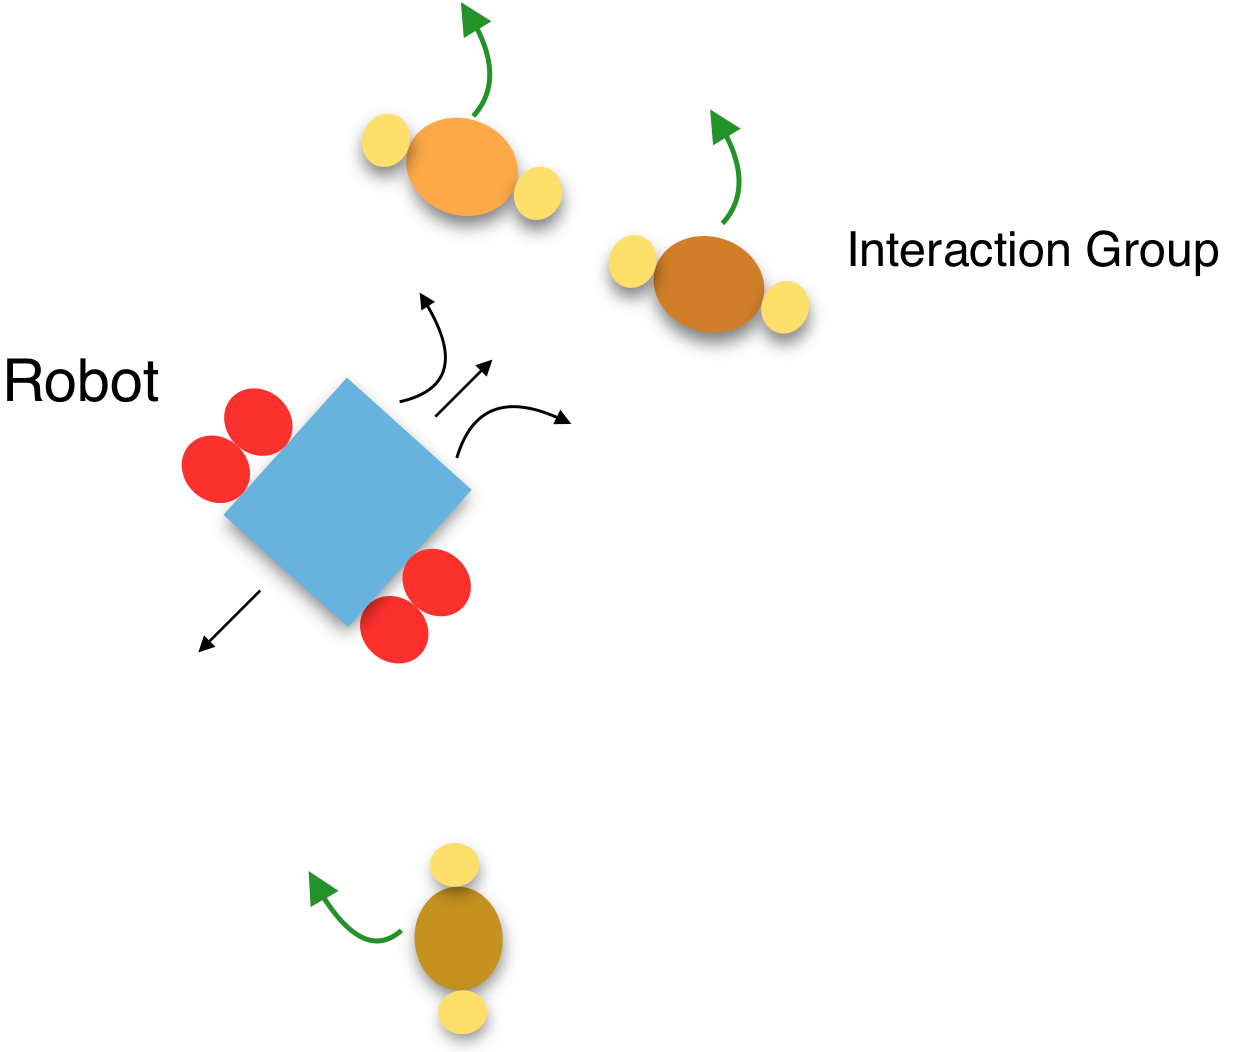
\includegraphics[scale = 0.15]{images/follow.png}
    \caption{Following}
    \label{fig:follow}
  \end{subfigure} 
  %\vspace{-3mm}
  \caption{The two tasks we consider, with arrows showing possible motion of the robot and people.}

    \vspace{-2mm}

  %\vspace{-3mm}
  \label{fig:behaviors}
  \end{figure}

\subsection{Following Task} 

In the second task, the interaction target(s) are moving and the robot should follow them. The robot should be able to deal with variability in the formation of the people it is following. Furthermore, it should be robust to false positive detections and be able to retain a following behaviour despite detecting other people who are in the scene but not relevant to the task. This task is shown diagrammatically in Figure \ref{fig:follow}. Following behaviours can be challenging because the robot's sensors often suffer from reliability issues as velocities increase \cite{kobilarov2006people}.

Previous work used an extended social force model enriched with a goal prediction module to allow a robot to walk side by side with a person \cite{ferrer2016robot}. The system tests different social forces parameters and allows the user to give feedback about the experience. Based on this feedback, the robot learns to adapt itself to the specific person.  Our work investigates the possibility of bypassing such models and simply learning the required behaviour robustly through data.  

Knox et al \cite{knox2013training} train a robot to perform several tasks that are similar to ours, such as maintaining a conversational distance and "magnetic control". However, training is done using human generated reward and reinforcement learning through the TAMER framework \cite{knox2009interactively}. Furthermore, in contrast to our work, their approach can handle only a single interaction target and assumes perfect sensing.

More generally, in social robotics settings, LfD is primarily used for learning high-level behaviours \cite{louie2016learning} \cite{lockerd2004tutelage}. Our work fills this gap, by showing how to learn low-level social robot control from demonstration. Outside of social settings, LfD is most commonly used for complex manipulation tasks \cite{argall2009survey}. Deep learning has also been used in an end-to-end fashion to perform behavioural cloning in self-driving cars \sw{cite}. However, such an approach is highly intensive in terms of both data and computation.  By contrast, we rely for people detection on a sensor fusion pipeline that uses both the RGBD camera and the laser rangefinders of the robot to enable $360^\circ$ tracking.  Consequently, we require only a modest amount of data ($\approx 1hr$), perform all processing on the robot, and cope successfully with the robot's limited RGBD field of view.

%Our work does not perform end to end learning for several reasons. Firstly, people detection modules are typically common to several robot functions such as navigation. Secondly learning end-to-end would require vast amounts of data as well as processing being offloaded to another machine. In contrast we only require a modest amount of data ($\approx 1hr$) and perform all processing on the robot. Finally the RGBD field of view of our robot is quite limited. People detection relies instead on a sensor fusion pipeline that uses both the RGBD camera and the laser rangefinders of the robot to enable $360^o$ tracking.  

\sw{Is this section about the problem setting or related work?  It seems to have morphed from one to the other.}

% Another crucial issue that we would like to address is that in many cases, even though the environment around the robot changes, there should be no change in the behavior of the robot. This \emph{invariance} is very hard to hard code. For example if we were to use a social force model to solve the tasks, the calculated forces would vary all the time based on the people position. This in turn means that the behavior of the robot could become either over or under sensitive depending on tuning. By learning these behaviors from demonstrations we hope that the robot will not only learn what to do and how to do it, but also when to do it.


\subsection{Data and Experiments \label{subsec:data_exp}} 

To collect that data required for learning, we performed one set of experiments for each of the tasks described above. Every experimental session involved two experimenters, one or more volunteers from the University of Amsterdam, and a TERESA\footnote{www.teresaproject.eu} intelligent telepresence system, shown in Figure \ref{fig:robot}.  One experimenter would act as the pilot while the other would be on the other side of the interaction and would have two roles. The first role would be to act as an interaction target. The second would be to instruct the volunteers to join or leave the interaction and attempt to change the shape of the interaction group (triggering an appropriate reaction from the pilot) in order to capture sufficient variability in the data.  

During these interactions, we record the positions and linear velocities of all people detected and tracked by the robot. We also record a binary label, indicating the primary interaction target for the robot. The primary interaction target is defined as the most important person in the interaction and it is defined by the pilot. The observation $o_t$ of $K$ people tracked at time $t$ where the first person is the primary interaction target is therefore defined as, $o_t = \{(\rho_1,\phi_1,\dot{\rho}_1,\dot{\phi}_1,1),... (\rho_,\phi_{K_t},\dot{\rho}_{K_t},\dot{\phi}_{K_t},0)\}_t$, where $\rho_k$ and $\phi_k$ are the distance and angle from the robot respectively and $\dot{\rho}_k$ and $\dot{\phi}_k$ represent the associated velocities. This is shown in Figure \ref{fig:data}. We in addition recorded the linear and angular velocity commands given by the pilot, $a_t = (v_t,\omega_t)$, where $a_t$ denotes the action at time $t$. Recording took place at 10Hz, which amounts to the control rate we would use for the robot.  It is also worth noting that these interactions took place in different environments each containing different amounts of people and different sources of false possitives for the people detection modules.

  	\begin{figure}[tbh]
	\centering
      \begin{subfigure}[b]{0.35\columnwidth}
          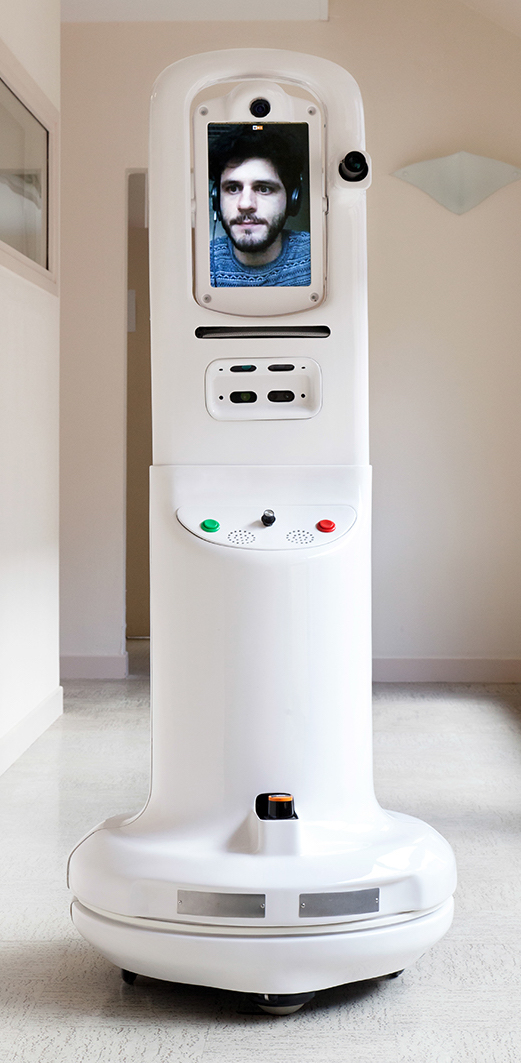
\includegraphics[scale = 0.15]{images/robot2.jpg}

    \caption{}
    \label{fig:data}
  \end{subfigure}
%  \hspace{2mm}
  \begin{subfigure}[b]{0.35\columnwidth}
%  \hspace{2mm}

    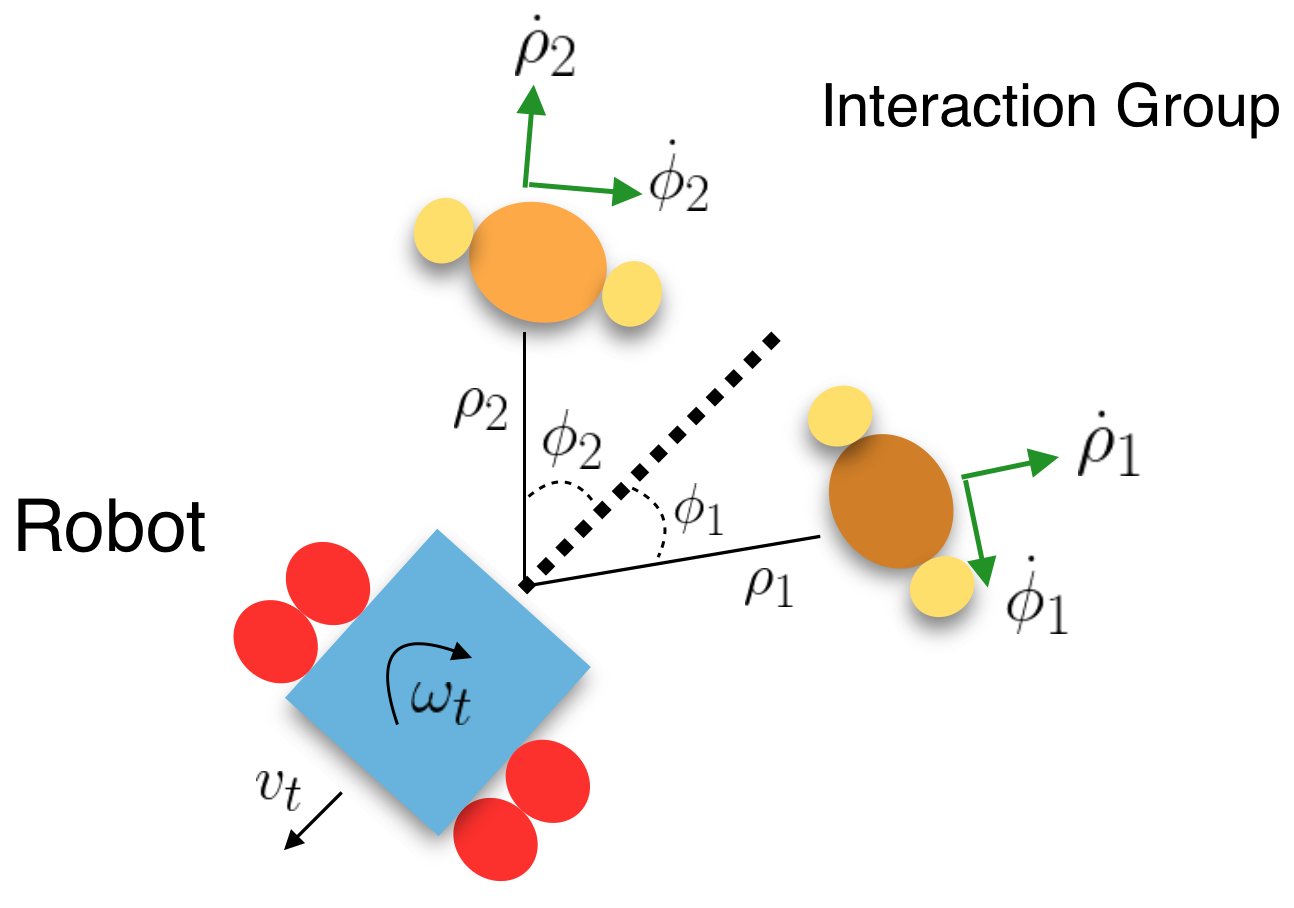
\includegraphics[scale = 0.19]{images/data.png}
  \vspace{5mm}
    \caption{}
       \label{fig:robot}
  \end{subfigure} 

  \caption{(a) The TERESA telepresence robot used in our experiments; (b) the data collected for a single frame $(t)$ during our experiments.}

    \vspace{-2mm}
  \label{fig:data_robot}
  \end{figure}

\section{Method}
In the previous sections we described the social tasks we will attempt to learn by demonstration. We have also described the data collection procedure that would allow us to do so. In this section we describe the learning architecture used to learn a mapping from robot observations to actions from this data. To derive this architecture we look closely into the data collected and the tasks at hand.
First we explain the type of learning we will perform namely, behavioral cloning, and argue that neural networks are an appropriate means of executing this learning procedure. We then build our network piece by piece by looking at different aspects of the data such as possible input representations, temporal aspects and the output mappings. 

\subsection{Behavioral Cloning}
There are several ways perform LfD in robots that have been studied extensively in the literature. The simplest and most straightforward of these is what is usually called behavioral cloning (BC). In BC we tackle LfD from a supervised learning (SL) perspective by treating the (sequences of) observations as input states $s_t$ and actions $a_t$ as labels, to train a \emph{policy} $\pi(s_t,a_t)$ so that similar actions are performed in similar situations. In this view any supervised learning paradigm (regression, classification) and algorithm (decision trees, gaussian processes, neural networks) \cite{bishop2006pattern} can be used to learn this policy from the data. Other forms of LfD exist, namely Inverse Reinforcement Learning \cite{abbeel2004apprenticeship} which attempts to extract a cost function from the demonstrations that is subsequently used to plan (or learn \cite{boularias2011relative}) a policy. IRL has been shown to be more data efficient and more transferable across environments. It is however harder apply in practice. IRL is certainly an interesting direction for future work however in this paper we use behavioural cloning because it is simpler and we are in possetion of enough data to perform learning.

Our choice of algorithm for learning the mapping function in this case is a Neural Network for two reasons. The first of these is \emph{generality}. In these paper our aim is to learn two (and potentially more) behaviours using a single algortithm. NNs can learn the features that are important for prediction automatically and this in turn means there would be therefore no need to define problem-specific features for a task, such as for example a group detection module. The second reason to use NNs is \emph{modularity}. This means that we can use different computation modules depending on our high level application. For example through recurrent neural networks we can easily deal with observations that vary (non linearly) over time in order to alleviate problems arising from noise in detections. Also in our input representation we have continuous as well as discrete variables, neural networks can deal with such representations easily. Finally, we are in this case outputing two values ($v,\omega$) and common supervised learning algorithms would treat each output independantly. This is ofcourse possible with methods other than neural networks, such as Gaussian Mixture Models (GMMs) or Hidden Markov Models (HMM), which would however require feature engineering to perform well.  

\subsection{Inputs and convolutional layers \label{subsec:meth_inp}}
In the previous section we have seen that our observations at time t can be formulated as:

\begin{equation}
 	o_t = \{(\rho_1,\phi_1,\dot{\rho}_1,\dot{\phi}_1,1),... (\rho_{K_t},\phi_{K_t},\dot{\rho}_{K_t},\dot{\phi}_{K_t},0)\}_t
\end{equation}
An important aspect of our observations is that the amount of people around the robot is dependent on time. This means that the size of our input vector would vary with time depending on the value of $K_t$. This is not very friendly for most learning algorithms that would expect a fixed input vector size. One way to alleviate this problem would be to fix $K$ to some number we consider reasonable. If the amount of people in the data is more than $K$ we would keep the $K$ closest. If the amount is smaller than $K$ we would simply fill the first $K$ positions of the vector and leave the last one with zeros. In this case however we are suggesting to the algorithm that there is a person on the robot since $\rho,\theta = (0,0)$. This could have adverse effects on learning, we could thus add another binary feature to our observation vector, to indicate wether the detection is a valid one. The new observation vector would thus look something like:

\begin{equation}
 	o_t = \{(\rho_1,\phi_1,\dot{\rho}_1,\dot{\phi}_1,1,1),... (\rho_{K_t},\phi_{K_t},\dot{\rho}_{K_t},\dot{\phi}_{K_t},0,0)\}_t
\end{equation}
Although perhaps inconvienient the above notation would give the learning algorithm all the information to learn a mapping. 

A more convienient representation however would be to imprint the observation on an image. This would involve fixing a maximum distance $x_{max},y_{max}$ from the robot and subsecuently painting all the people around the robot within that area on a ternary image. That is an image of three possible values, $0=$ no person is present, $1=$ a person is present, $2=$ a primary interaction target is present. We also denote the velocities of people as lines extending from the detections in the direction of the detected velocity and with a length that is representative of its magnitude. An example of such an image is shown in Figure \ref{fig:state}. Another convienient aspect of this representation is that our image can contain further information such as for example the nearest non-human obstacles and the orientation of the people if this can be reliably detected. 

Although more convienient however this representation comes with a clear setback, which is that we are increasing the dimensionality of the problem. Usually when learning we seek to reduce the dimensionality of the problem through feature engineering, here we are in a sense doing the opposite. 

To alleviate this setback we use convolutional neural networks (CNN) on this input representation. CNNs perform very well on spacially structured input such as the one at hand where although the actual dimentionality of the input is large, the possible images that can take place are limited and their features can be learned. CNNs are also very useful because they are able to build invariances. This is extremely helpful in this application because the network can learn to ignore some configurations of the input making learning more robust. Our analysis in the next section we show that in practice this representation along with CNNs is not only more convienient but also beneficial to learning and stability of the resulting behaviour.

  	\begin{figure}[tbh]
  	\centering
      \begin{subfigure}[b]{0.30\columnwidth}
    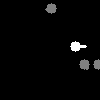
\includegraphics[scale = 0.80]{images/state1.png}
    \label{fig:state1}
  \end{subfigure}
  \begin{subfigure}[b]{0.30\columnwidth}
    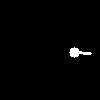
\includegraphics[scale = 0.80]{images/state2.png}
       \label{fig:state2}
  \end{subfigure} 
    \begin{subfigure}[b]{0.30\columnwidth}
    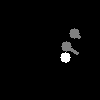
\includegraphics[scale = 0.80]{images/state3.png}
       \label{fig:state3}
  \end{subfigure}
  %\vspace{-3mm}
  \caption{Example images representing the state of the robot. Circles denote people, lines denote velocity. The white circle represents the primary interaction target.}

    \vspace{-2mm}
  \label{fig:state}
  \end{figure}

\subsection{Dynamics and long short term memory}
Using a single observation as input to a convolutional neural network that outputs a control is unlikely to succesful for three main reasons.

\begin{itemize}
\item A single observation instance $o_t$ does not contain higher order information such a the acceleration of people.
\item The people detection module is not perfect. False positives and negatives are common within the data, not having context information from previous observations will affect robustness of the controller.
\item The velocity information (albeit helpful) is innacurate and noisy.
\end{itemize}

Long-short term memory \cite{hochreiter1997long} is a de-facto standard way of dealing with time depdendent output and partial observability when NNs are applied to decision making \cite{schmidhuber2015deep}. The LSTM is a type of Recurrent Neural Network (RNN) i.e., a neural network that can process time dependent inputs. In contrast with vanilla versions of RNNs however and LSTM is robust to unstable gradient phenomena often encountered during training of deep networks. In our architecture we use LSTMs to deal with the time dependent nature of the problem and achieve robustness in the face of uncertain detections.



\subsection{Outputs and Overall Architecture}
After processing by the recurrent layers the architecture then outputs two real continuous values representing the linear and angular velocities ($v_{pred},\omega_{pred}$) of the robot. Another solution would be to discretise the outputs and treat the prediction as a classification problem. While doing so has some benefits allowing us to predict multimodal output distributions, we chose regression for two reasons. First, there is no requirement to define the discretisation for each task allowing the architecture to remain more general, second continuous outputs bring about potentialy smoother behaviour. In order to train our network we use the mean squared error (MSE) between the network's prediction and the data and train using backprogapation using the Adam \cite{kingma2014adam} optimisation routine. The resulting architecture can be seen in Figure []. We employ three convolutional layers consisting of 10 3x3 filters at each layer. We use ReLU non-linearities followed by a subsampling step using max-pooling of size 2. The output from the last convolutional layer is flattened and processed through two LSTM layers of size 200 and 100 respectively. Finally a densely connected layer is used to output the two required control values. 
 
A final crucial point is that prediction needs to happen at 10Hz on a conventional computer, such as the one used by our robot. The proposed architecture would run comfortably on an Intel i7 processor at the required control rate.


% \subsection{Continuous Learning Pipeline}
% One major setback of behavioural cloning that has been studied in the literature, is that since most demonstrations are noisy examples of what the robot should do, the robot never learns how to get out of difficult situations when it finds itself in one, because it was never encountered in the data. For this reason we take a similar approach to the one encountered in []. First we collect some data using the robot, perform learning and deploy the learned policy on the robot. During execution we correct the robot whenever it makes a mistake, record the data from the intervention and then hand the control back to the robot.


\section{Evaluation and results}
In order to evaluate our proposed architecture we will compare it against three other learning baselines. The first of these is an off-the-shelf regression method. In this case due to the mixed types in the inputs we will use Gradient Boosting Regression (GBR), which along with other ensemble methods is considered one of the best off the shelf algorithms for non-linear regression. We use this baseline to show that for traditional regression methods to work well task specific feature engineering would need to be performed. Input to this baseline are the concatenated observation vectors for K people around the robot (as described in the begining of Section \ref{subsec:meth_inp}) for T timesteps. In this case K=4 and T =5 so theinput vector representations is $K\times T \times 6 = 120$. We did not use T=20 as in our method since the explosion in input space caused a degradation in performance. The second baseline we use is an architecture that omits the convolutional layers and only employs the LSTM layers. The input representation is a vector concatenating the features of K people around the robot where K in this case is set to 4. Our third baseline is an architecture with no memory and only uses the convolutional layers.

To measure performance we are not simply concerned about how well the algorithms fit the data but also how they perform when placed on the robot and tested with humans. Therefore to evaluate we use a mixture of quantitative and qualitative metrics. 

\subsection{Mean squared error}
As mentioned in the previous section, the objective function used to learn the mapping between observations and controls is the MSE. A first measure of the performance of DBSoC and the proposed baselines is to measure the MSE for a test dataset not used during learning. In our case the test set was comprised of 20\% of the data for each task which amounts to 8543 and 5643 datapoints for the follow and group reconfiguration tasks respectively. Table \ref{tab:mse} documents the performance of each method on both the training and test sets. We can see that DBSoC outperforms all baselines on the test set, followed by the LSTM method, (where no image representation is used). GBR is the worse performer by a significant margin.

% \begin{table}[]
% \centering
% \caption{Mean squared error rates for our full model and the prosposed baselines. The error is computed on 20\% of the data held out for testing purposes in each case.} \label{tab:}
% \label{my-label}
% \begin{tabular}{|l|l|l|l|l|}
% \hline
%        & GBR  & LSTM & Short & DBSoC \\ \hline
% Group  & 0.1 & 0.015 & 0.0126  & \textbf{0.0084}       \\ \hline
% Follow & 0.1 & 0.0063 & 0.0149  & \textbf{0.0055}       \\ \hline
% \end{tabular}

% \end{table}

\begin{table}[]
\centering
\caption{Mean squared error rates for our full model and the prosposed baselines. The error is computed on 20\% of the data held out for testing purposes in each case.}
\label{tab:mse}
\begin{tabular}{|c|c|c|c|l|c|}
\hline
                &             & {\ul GBR} & {\ul LSTM} & {\ul CONV} & {\ul DBSoC} \\ \hline
\textbf{Group}  & {\ul Train} & 0.0232     & 0.0098      & 0.0087     & \textbf{0.0018}  \\ \hline
                & {\ul Test}  & 0.0264     & 0.0120      & 0.015    & \textbf{0.0031}  \\ \hline
\textbf{Follow} & {\ul Train} & 0.0265    & 0.00334      & 0.0079     & \textbf{0.0030}  \\ \hline
                & {\ul Test}  & 0.0323     & 0.00450       & 0.0250    & \textbf{0.0036}  \\ \hline
\end{tabular}
\end{table}


\subsection{Output distribution}
A more qualitative yet insightful means of evaluation can be achieved by examining the output distribution on the outputs of each learned policy given the inputs. That is, using a portion of the validation data we plot the predicted linear and angular velocities ($v_{pred},\omega_{pred}$) and compare them with the actual values encountered in the data $v_{dem},\omega_{dem}$. This gives an idea as to how the output disribution of the predictor matches that of the human demonstrator. This can be more insightful than a single metric value since it can give as an insight on the expected behaviour of the robot. Figures \ref{fig:data} overlays the $v_{dem},\omega_{dem}$ (blue) with $v_{pred},\omega_{pred}$ for our method and the baselines for the follow task. The most obvious observation is that GBR captures the demonstrated distribution very badly. Its behaviour is extected to not use large angular velocities (y-axis) and will thus be not very responsive. In addition there seems to be a lot of uncertainty around the origin, possibly leading to oscilatory behaviour between positive an negative velocities. The short memory architecture also seems unable to capture the distribution, we see a lot of points that are scattered and far away from any data point we can thus also expect relatively poor behaviour. The LSTM policy on the other hand seems to have similar capabilities to DBSoC which clearly does a very good job at matching the demonstrators outputs. 



  	\begin{figure}[tbh]
      \begin{subfigure}[b]{0.45\columnwidth}

    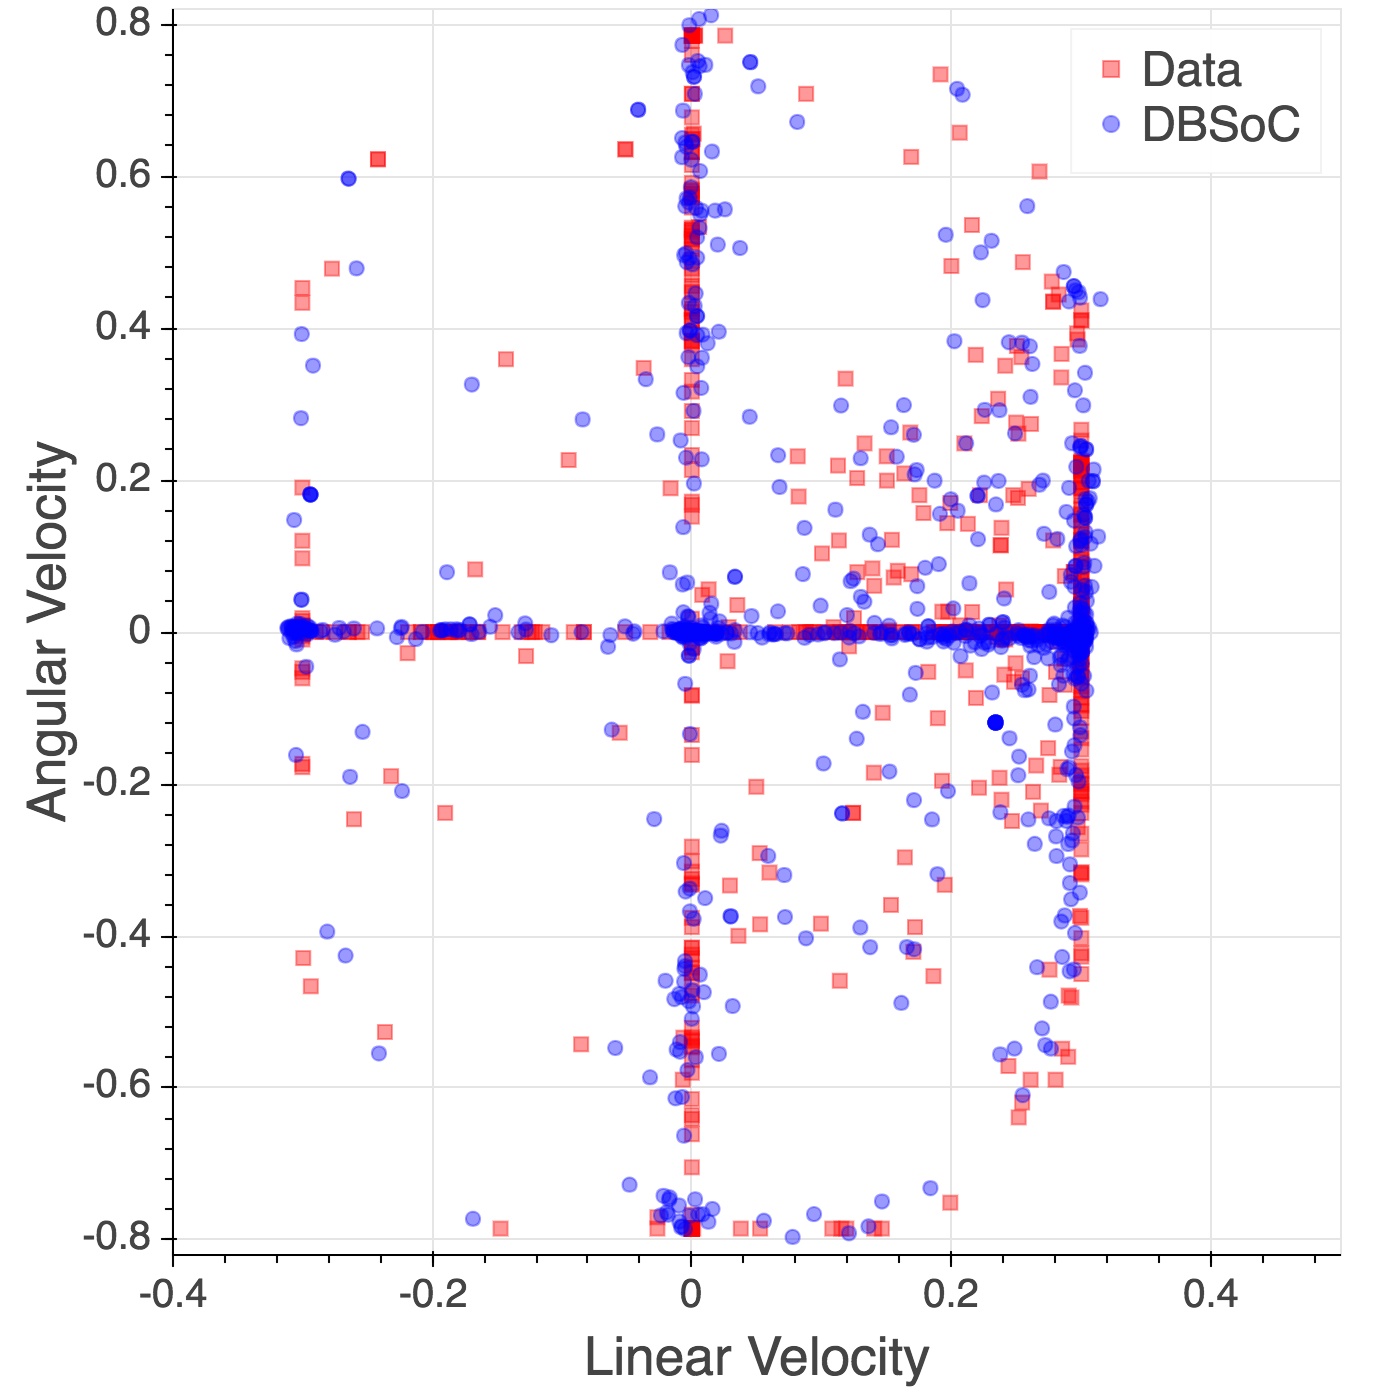
\includegraphics[scale = 0.09]{images/full_dist.png}
    \caption{DBSoC}
    \label{fig:data}
  \end{subfigure}
    	\hspace{5mm}
  \begin{subfigure}[b]{0.45\columnwidth}

    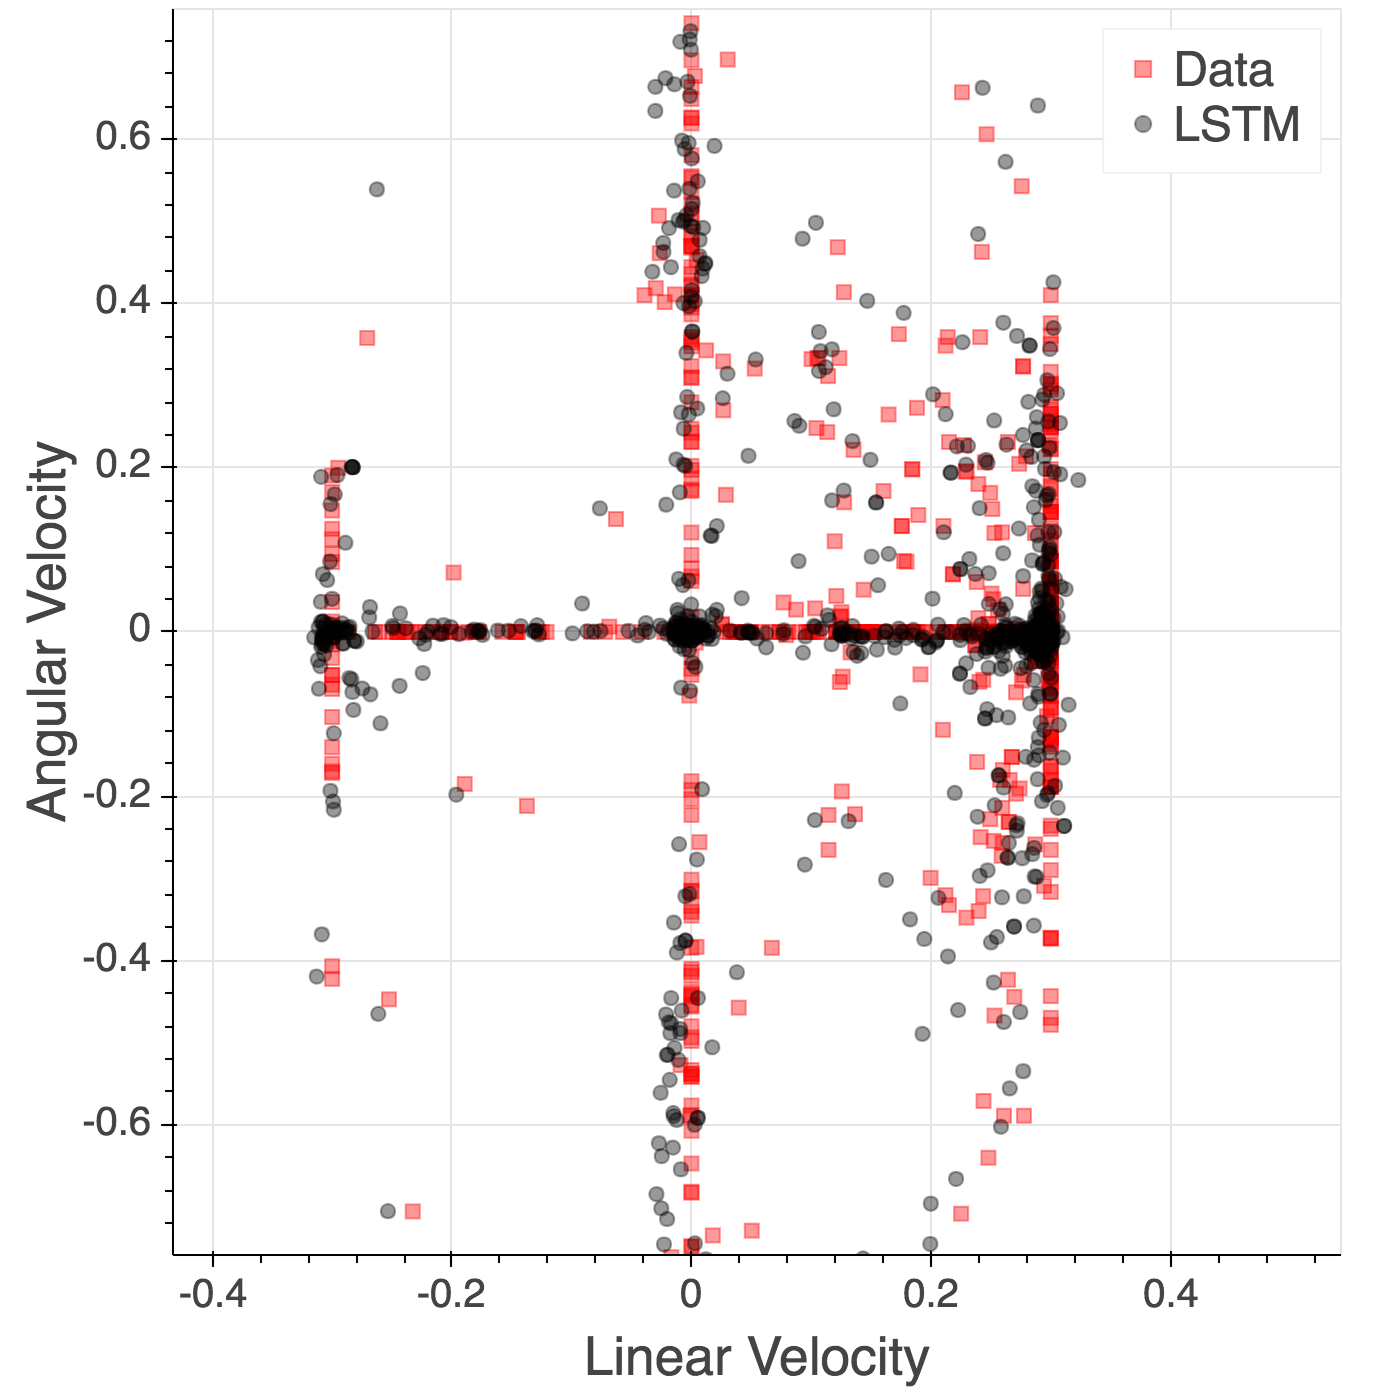
\includegraphics[scale = 0.09]{images/lstm_dist.png}
    \caption{LSTM}
       \label{fig:robot}
  \end{subfigure} 
  \\
        \begin{subfigure}[b]{0.45\columnwidth}
    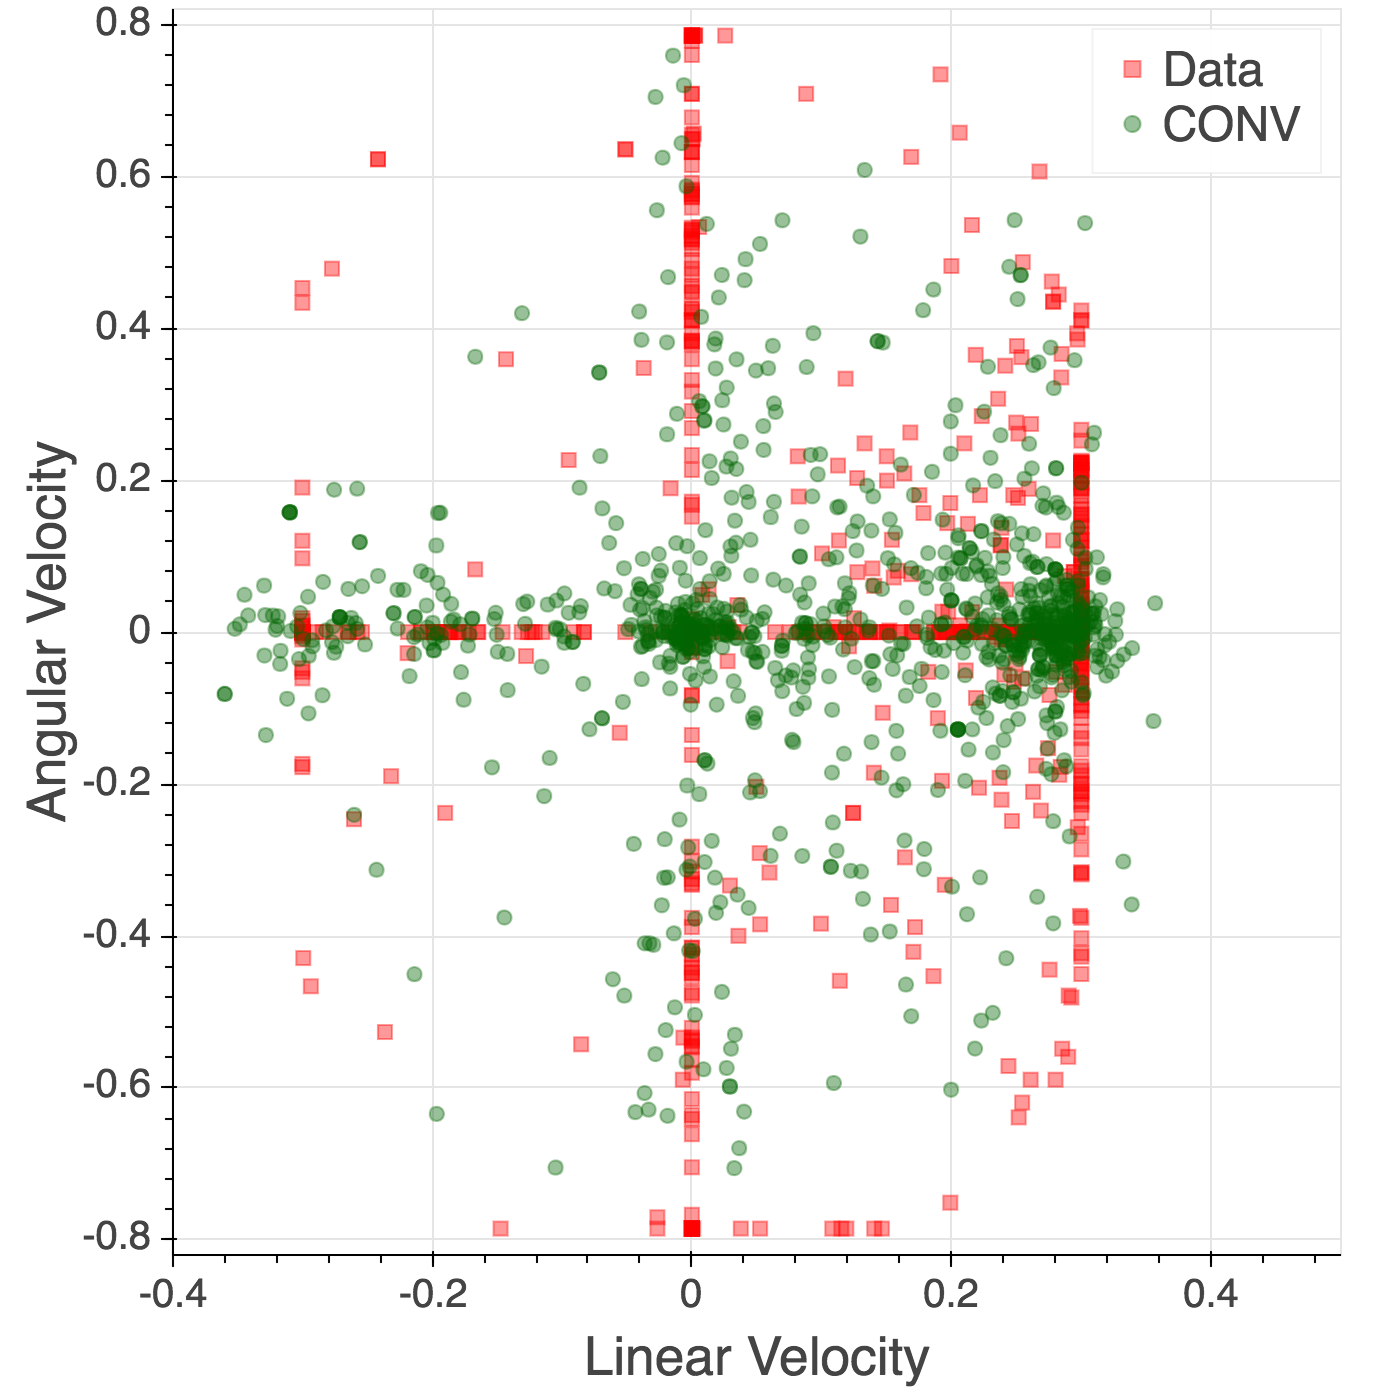
\includegraphics[scale = 0.09]{images/short_dist.png}
    \caption{CONV}
    \label{fig:data}
  \end{subfigure}
  \hspace{5mm}
  \begin{subfigure}[b]{0.45\columnwidth}
    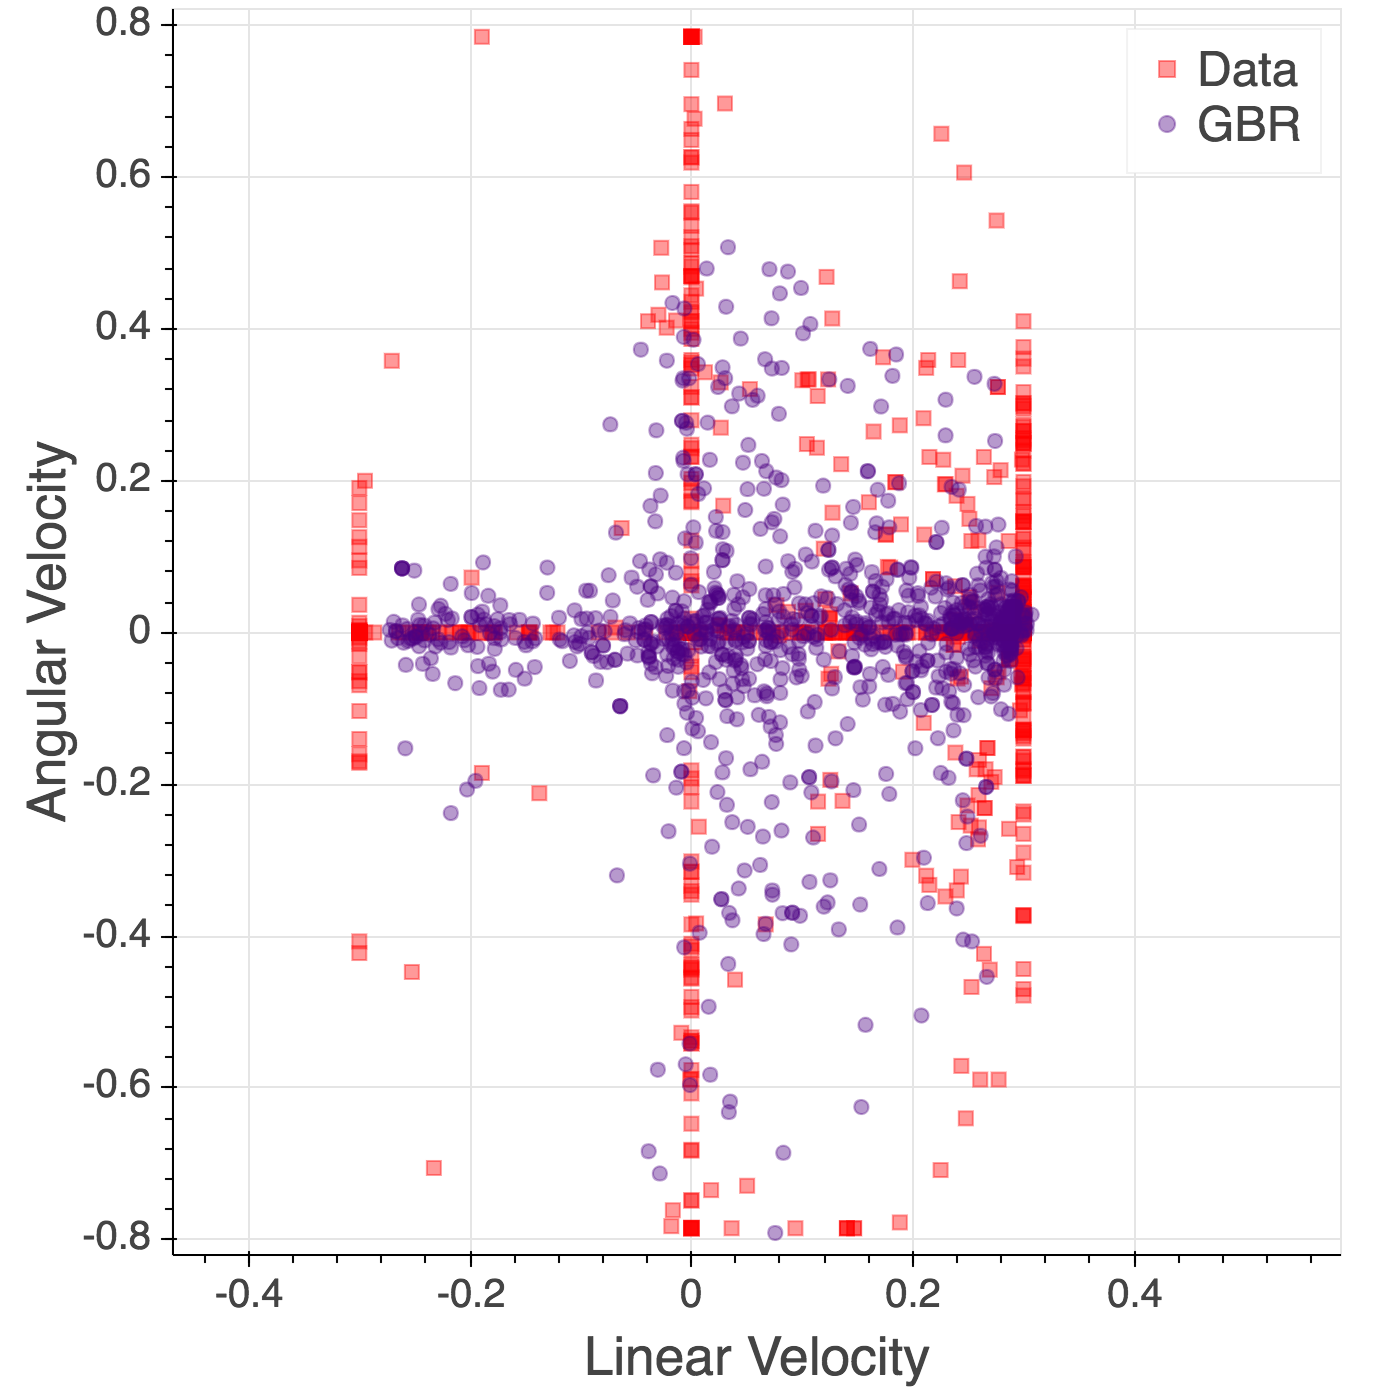
\includegraphics[scale = 0.09]{images/gbr_dist.png}

    \caption{GBR}
       \label{fig:robot}
  \end{subfigure} 
  %\vspace{-3mm}
  \caption{Output disributions of Follow data (red) and learned policies.}

    \vspace{-2mm}
  \label{fig:data_robot}
  \end{figure}


\subsection{Human evaluation}
This paper is a contribution to making social robotic behaviours easier to program. The end product of such an effort must then be evaluated by humans. Also unless a policy is deployed on an actual robot there is little way of knowing how it performs. This is because while the problem is tackled from a supervised leanring perspective it is still a sequential decision making problem. This means that an action of the robot affects its environment and wrong actions at the wrong time might bring the robot to states it does not know how to recover from.

Our human evaluation in this case consisted of groups of subjects from the University of Amsterdam interacting with the learned policies as well as a hard-coded controller. This hard-coded behaviour would take the person closest to the person and attempt to keep a constant distance ($\rho$) of $1.3m$, in accordance with standard proxemics [hall], and an orientation ($\phi$) of $0^o$. The subjects were first briefed about the purpose of each behaviour they were about to evaluate (i.e., follow or group conversation). Following the briefing was a calibration step where the subjects were shown human level performance in each of the tasks as well as various policies at random. This allowed the subjects to get a feel as to what they should expect from the robot. After calibration the subjects were given about 2 minutes to interact with each policy to be evaluated at each of the tasks. The policies were given anonymously and at different order each time. The subjects were then given the opportunity to rate the social performance of each policy with a number from 1 to 10, with 10 being human level performance. Examples of the interactions for different tasks and policies in such an evaluation session can be seen in the attached video.

A summary of the scores for each policy in question are shown as box plots in Figure \ref{fig:human}. The first observation we make is that different methods perform quite differently depending on the task. We can see for example that the hard-coded controller is percieved to perform very well for the follow behaviour - due to its smoothness of control - whereas in the group interaction task the controller performs more poorly. A common comment was that it would only concentrate on one person and would not adjust to the group. A perhaps more surprising result in that humans percieve GBR to be still a relavitely good policy on average. These ratings are noisy however because the behaviour would vary a lot depending on the situations that would arise in the interaction. In therms of DBSoC, a key observation is that it performs quite well during all evaluations. This is apparent from the fact that during no evaluation did it recieve a lower score than 5 while most methods did. On the other hand it did not manage to perform as well as the hard-coded controller on the follow task. This was mainly because control was less smooth for DBSoC as for all other baselines that employed learning.

During the course of these evaluations it became apparent how difficult it is for humans to evaluate social robotic behaviour. Perhaps a more detailed questionaire and more structured interaction scenarios would have been more appropriate to analyse the preferences of the subjects however this was not performed due to time constraints. Therefore while we do not consider these numbers to be hard evidence for the superior performance of our method they do support the generality and effectiveness of our approach. Furthermore, the fact that the subjects were allowed to interact freely with the robot suggest that results in Section are not a product of overfitting due to the nature of the collected data. 

	\begin{figure}[tbh]
      \begin{subfigure}[b]{0.40\columnwidth}
    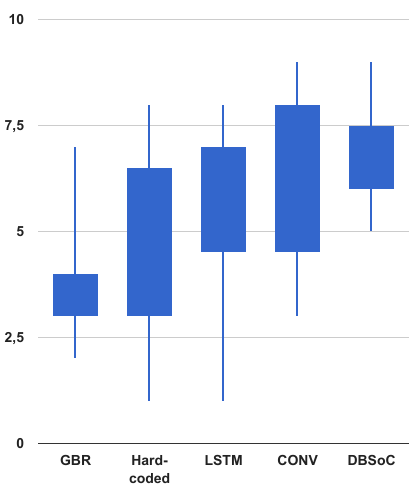
\includegraphics[scale = 0.30]{images/group_candle.png}
    \caption{Group Reconfiguration}
    \label{fig:static-res}
  \end{subfigure}
  \hspace{5mm}
  \begin{subfigure}[b]{0.40\columnwidth}
    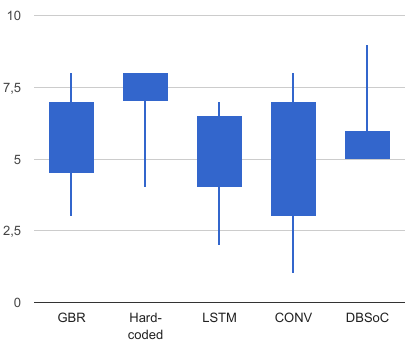
\includegraphics[scale = 0.30]{images/follow_candle.png}
    \caption{Following}
    \label{fig:follow}
  \end{subfigure} 
  %\vspace{-3mm}
  \caption{Box plots summarising human evaluation scores for all baselines on the two tasks.}
  %\vspace{-3mm}
  \label{fig:human}
  \end{figure}


\section{Conclusions and future work} 

\bibliographystyle{IEEEtran}
\bibliography{references}



\end{document}
